\documentclass[conference,compsoc]{IEEEtran}
\usepackage{graphicx}
\usepackage[spanish,es-tabla]{babel}
\usepackage[T1]{fontenc}
\usepackage{fontspec}
\usepackage{listings}
\usepackage{svg}
\usepackage{anyfontsize}
\usepackage{hyperref}
\graphicspath{ {figures/} }
\hypersetup{colorlinks = false}
\lstset{language=SQL,morekeywords={PREFIX,java,rdf,rdfs,url,@prefix}}
\newcommand{\rdf}{\textit{RDF}\ }
\newcommand{\spql}{\texttt{SPARQL}\ }

\begin{document}

\title{SUGERENCIAS PARA LA CONSTRUCCION DE CONSULTAS SPARQL, UNA ALTERNATIVA OPEN SOURCE\\ \ \\PROPUESTA}

\author{
    \IEEEauthorblockN{Carlos Andrés Ponce Godoy}
    \IEEEauthorblockA{\textit{Departamento de Informática} \\
    \textit{Universidad Técnica Federico Santa María}\\
    Valparaíso, Chile\\
    carlos.ponce@sansano.usm.cl}
}

\maketitle

\IEEEpubidadjcol

\begin{abstract}
    Here goes your abstract
\end{abstract}

\begin{IEEEkeywords}
    SPARQL, Web Semántica, RDF
\end{IEEEkeywords}

\IEEEpeerreviewmaketitle

\section{Definición del problema}

La web semántica es un conjunto de extensiones para la \textit{World Wide Web},
desarrolladas por el \textit{World Wide Web Consortium (W3C)} para permitir que
la información disponible en la internet puerda ser procesada por máquinas \cite{berners2001semantic}.

Para lograr esto, la web semántica propone agregar a la información ya existente
metadatos semánticos para que estos puedan ser procesados por agentes inteligentes,
los cuales obtendran esta información sin operadores humanos. Estos metadatos pueden
ser descritos utilizando multiples estandares existentes, uno de ellos es el 
\textit{Resource Description Framework (RDF)}, el cual define una estructura para
definir relaciones entre entidades \cite{world2014rdf}.

Estas relaciones se describen a través de un trio \textit{sujeto - predicado - objeto},
en el cual, cada uno de los elementos esta representado por un \textit{Uniform Resource Locator (URL)}.
Estas relaciones descritas en \rdf pueden ser visualizadas a través de grafos dirigidos como
el que se encuentra en la figura \ref{fig:rdf-graph1}

\begin{figure}%[h]
    \centering
    \includesvg[width=\linewidth]{rdf-graph.svg}
    \caption{Un grafo \rdf con dos nodos \textit{Subject} y \textit{Object} concetados a través de
    la relación \textit{Predicate}.}
    \label{fig:rdf-graph1}
\end{figure}

Un conjunto de multiples trios que describen multiples relaciones para una gran cantidad
de entidades se almacena en una \textit{Triplestore}, la cual consiste en una base de datos
diseñada para responder a consultas al estilo \textit{sujeto - predicado - objeto} del 
formato \rdf \cite{rusher2001triple}.

El lenguaje utilizado para obtener datos e información desde una \textit{Triplestore} es
\spql y su nombre corresponde a un acronimo recursivo, el cual significa \textit{SPARQL
Protocol and RDF Query Language} \cite{world2013sparql}.

El ejemplo más basico de una consulta \spql es el que utiliza las sentencias \texttt{SELECT}
y \texttt{WHERE}. Primero, definimos nuestro conjunto de datos en el bloque de código \ref{lst:basic-rdf}.

\begin{figure*}
    \begin{lstlisting}[captionpos=b, caption=Datos en formato \rdf., label=lst:basic-rdf, basicstyle=\ttfamily,frame=single]
@prefix exbook: <http://example.org/book>
@prefix purl: <http://purl.org/dc/elements/1.1>

exbook:book1 purl:title "SPARQL Tutorial" .
     \end{lstlisting}
\end{figure*}

Luego, realizamos la consulta con las siguientes sentencias, como se puede observar en
el segmento de código \ref{lst:basic-sparql}.

\begin{figure*}
    \begin{lstlisting}[captionpos=b, caption=Consulta SPARQL basica., label=lst:basic-sparql, basicstyle=\ttfamily,frame=single]
PREFIX exbook: <http://example.org/book>
PREFIX purl: <http://purl.org/dc/elements/1.1>
SELECT ?title
WHERE {
    exbook:book1 purl:title ?title .
}
     \end{lstlisting}
\end{figure*}

En base a nuestro conjunto de datos disponible, solo existe una
solución al patron de grafo descrito en la consulta, el resultado es la tabla \ref{tab:basic-result}.

\begin{table}[h]
    \label{tab:basic-result}
    \caption{Resultado de una consulta SPARQL básica}
    \centering
    \resizebox{0.5\linewidth}{!}{\begin{tabular}{|c|}
    \hline
    title               \\ \hline
    "SPARQL Tutorial"   \\ \hline
    \end{tabular}}
\end{table}

En base a todo lo anterior, podemos notar que escribir este tipo de consultas no es
sencillo e implica un esfuerzo cognitivo importante. Actualmente, si una persona
quisiera realizar una consulta a una \textit{Triplestore} o base de datos con soporte \spql, necesitará
conocer dos cosas, la sintaxis de \spql y la estructura de la base de datos que estamos
consultando.

Para apoyar a los nuevos usuarios a satisfacer estas dos necesidades, se han desarrollado
herramientas y plataformas que facilitan la construcción de consultas y la exploración
de las entidades en las bases de datos \rdf como por ejemplo, \textit{RDFExplorer}
\cite{vargas2019rdf}, \textit{Tabulator} \cite{berners2006tabulator} , \textit{Explorator}
\cite{araujo2009experimenting}, \textit{DBpedia Atlas} \cite{valsecchi2015dbpedia},
\textit{RDF Visualizer} \cite{sayers2004node}, \textit{SPARQL Assist}
\cite{mccarthy2012sparql} o \textit{YASGUI} \cite{rietveld2017yasgui}.

Estas herramientas nos facilitan la tarea de explorar los contenidos de la base de datos \rdf
y además nos permiten construir consultas \spql de forma interactiva. Para nuestro trabajo,
hemos decidio trabajar con la plataforma \textit{RDFExplorer} (figura \ref{fig:rdfexplorer}) debido a las siguientes
caracteristicas que presenta:

\begin{itemize}
    \item Facilidad de usó.
    \item Construcción interactiva de consultas \spql.
    \item Navegación de entidades en la base de datos.
    \item Generación de resultados parciales.
    \item Código fuente disponible y abierto.
\end{itemize}

\begin{figure*}
    \centering
    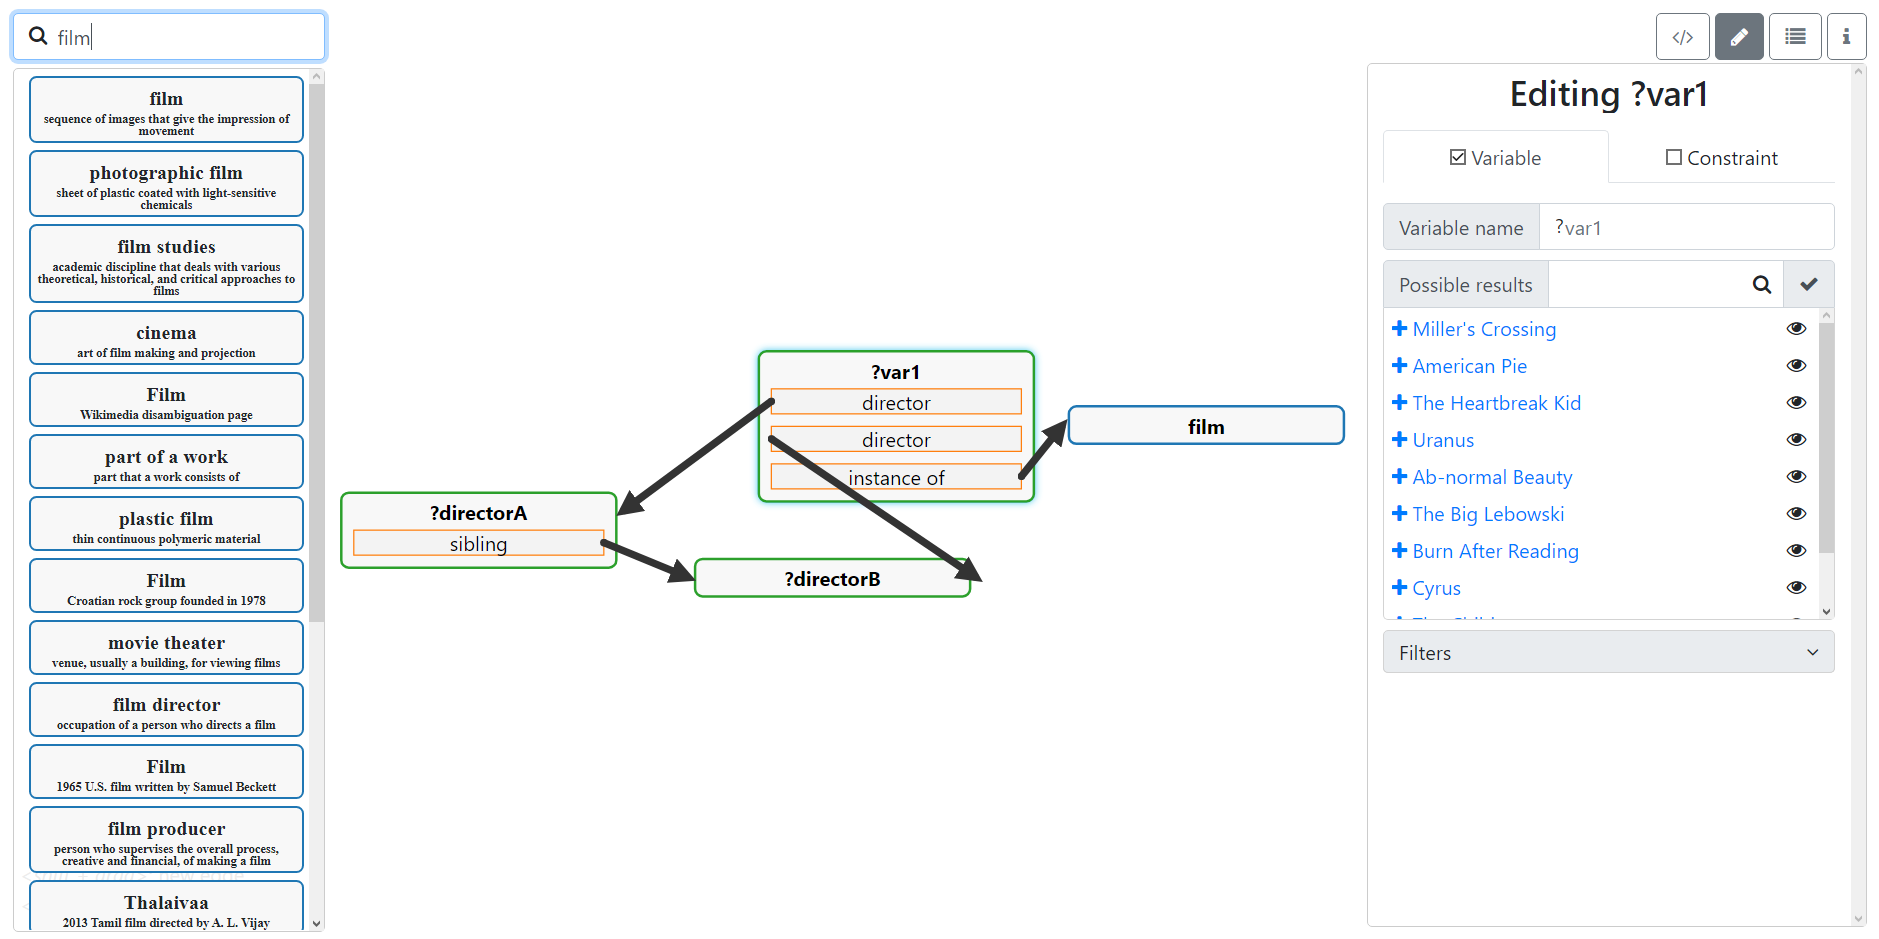
\includegraphics[width=\linewidth]{rdfexplorer.png}
    \caption{RDF Explorer}
    \label{fig:rdfexplorer}
\end{figure*}

Sin embargo, aun cuando utilizamos herramientas como \textit{RDFExplorer}, debemos tener
algún grado de conocimiento sobre las propiedades de las entidades disponibles
en la base de datos, los cuales no tenemos cuando somos nuevos usuarios.

Una forma de apoyar a estos usuarios en la tarea de descubrir las propiedades disponibles
en nuestra \textit{Triplestore} es generar recomendaciones o sugerencias sobre los \textit{predicados}
disponible para una determinada entidad, esto es similar a lo realizado por herramientas de autocompletado
al escribir documentos o lo que es más cercano al campo de la programación y la informática, el
autocompletado de código realizado por entornos de desarrollo integrados \cite{bruch2009learning}.

Actualmente, existen soluciones y herramientas que nos permiten obtener recomendaciones en base a 
consultas \spql incompletas como \textit{Gosparqled} \cite{campinas2014live}, \textit{LinkedWiki editor}
\cite{rafes2018designing}, \textit{SPARKLIS} \cite{ferre2017sparklis}, \textit{SPACE} \cite{kramer2013space}
y \textit{SPARQLforHumans} \cite{parra2020autocompletion}.

De las anteriores alternativas, la unica que actualmente se encuentra integrada con \textit{RDFExplorer}
es \textit{SPARQLforHumans}. Sin embargo, esta solución tiene un problema fundamental, su implementación
se ha realizado utilizando el lenguaje de programación $C\#$ y el framework \texttt{.NET} en el sistema
operativo \textit{Windows} lo cual limita los entornos de ejecución disponibles en los que puede ser utilizado,
debido a que depende directamente de las bibliotecas \textit{DLL} del proyecto \textit{Apache Lucene}
\cite{bialecki2012apache}.

% si bien actualmente los componentes del framework se encuentran bajo las licencias MIT o Apache 2, 
% la propiedad sigue perteneciendo a la empresa Microsoft, la cual, es conocida por su compleja historia
% con la comunidad de código abierto.

En base a todo lo expuesto anteriormente, con este trabajo buscamos replicar la funcionalidad obtenida por
el proyecto \textit{SPARQLforHumans} pero con una restricción importante, los componentes de nuestra arquitectura
solo pueden corresponder a software gratuito y de código abierto. Además, buscamos realizar las siguientes mejoras
al rendimiento global del sistema:

\begin{itemize}
    \item Reducir el tiempo de procesamiento para los dumps de la base de datos de Wikipedia.
    \item Reducir el tiempo necesario para generar una recomendación a una consulta \spql incompleta.
\end{itemize}

\section{Objetivos}

    \subsection{Objetivo general}

Diseñar e implementar un sistema que permita obtener sugerencias para el posible
resultado de una consulta SPARQL incompleta utilizando exclusivamente
componentes de código abierto.

    \subsection{Objetivos especificos}

\begin{itemize}
    \item Diseñar el mecanismo de recomendación para las entidades de una consulta.
    \item Diseñar la arquitectura del sistema utilizando solamente componentes de código abierto.
    \item Implementar la arquitectura propuesta.
    \item Evaluar el rendimiento de la solución implementada.
\end{itemize}

\section{Discusión bibliográfica preliminar}

Para abordar nuestro problema primero debemos aclarar algunos conceptos que han sido
mencionados en las secciones anteriores, tales como la web semántica, SPARQL, RDF y el
contexto en el que estos se utilizan. Para esto, nos apoyaremos en las siguientes definiciones.

    \subsection{La web semántica}

La red informática mundial, \textit{World Wide Web} o simplemente \textit{Web} es el sistema de información público más importante
desarrollado en los últimos 30 años, el cual permite la transmisión de documentos electrónicos identificados
por \texttt{URLs} \textit{(Uniform Resource Locators)}, los cuales pueden estar enlazados a otros documentos 
a través de \texttt{hipertexto} y que se encuentran disponibles utilizando servicios de la internet.

La \textit{World Wide Web} fue diseñada como un espacio para la información con el objetivo de no solo ser
útil para las comunicaciones entre humanos, sino que también un lugar donde las máquinas podrían ayudar y participar.
Sin embargo, uno de los principales problemas de la \textit{Web} es que la mayor parte de su contenido ha sido
diseñado para ser consumido por humanos, lo que implica que para las máquinas y el software no es fácil acceder 
e interpretar el contenido disponible, incluso si este proviene de una base de datos estructurada a través de
columnas claras y tipificadas. La web semántica busca desarrollar herramientas,
lenguajes, protocolos y estándares que permitan, tanto a maquinas como humanos, procesar toda la información disponible en la
\textit{Web}. En base a esto, podemos definir a la web semántinca como la idea de generar
una red de datos en la \textit{Web}, hasta cierto punto, una base de datos global. \cite{berners1998semantic}

    \subsubsection{Arquitectura de la web semántica}

[INSERTAR IMAGEN DE WIKIPEDIA]

    \subsection{RDF}

    RDF is...

    \subsection{SPARQL}

    \section{Plan de trabajo}

    \section{Arbol del problema}

\bibliographystyle{IEEEtran}
\bibliography{IEEEabrv, propuesta.bib}

\end{document}

% refs: what is sparql
% refs: what is rdf
% refs: what is wikidata
% refs: ides, autocompletion features, intellisense